\documentclass{../template/texnote}

\title{\textbf{How to Improve your ML models}}[author={Linn Abraham}]

\begin{document}
    \maketitle \currentdoc{note}
    %<*note>
\section{Introduction}
The primary goal of developing a machine learning model is to be able to learn from training samples and 
generalize this learning to real world samples.
When developing machine learning models, you are often in a better situation if your model is overfitting rather than if its underfitting.
That is why achieving overfitting is in itself considered an achievement or rather as a first step towards making progress.
When we talk about generalization we talk about a model that is overfit.
%The term generalization is often used in an opposite sense to on overfit model.
%Improving the performance of your ML models is the primary concern of an ML developer.
How do we improve the performance of an overfitting model or rather how do we improve the generalization of our network?
But before answering that, let us ask ourselves why Machine Learning or Deep Learning works at all?
Is Machine Learning just glorified interpolation or is there even any relation between the two?
Understanding the answer to these would also allow us to appreciate how human intelligence is seen to 
better than this so called machine intelligence.
%What can be done to improve the performance of your models?
We will also come to certain practical considerations for improving the generalization of our models.
    \begin{figure}
    \begin{center}
        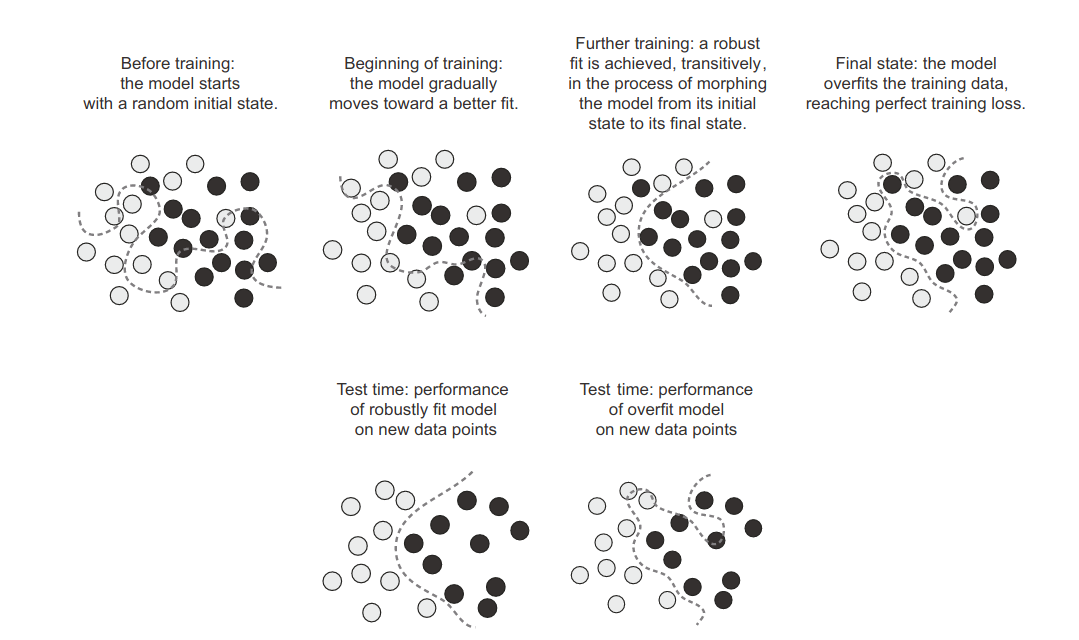
\includegraphics[scale=0.3]{Linn/overfitting_chollet.png}
    \end{center}
    \caption{Top panel shows how a model goes from underfit to overfit. The bottom panel shows how the two different models perform on test data. Image Credit: Francois Chollet.}
    \label{fig:overfit}
    \end{figure}
    
\section{Generalization in ML models}
Consider the input space in a problem as simple as the MNIST classification problem. The images here are $28 \times 28$ arrays of integers between 0 and 255.
The total number of elements in the input space, which is 256 to the power of 784, is much greater than the number of atoms in the universe.
Whereas the number of training samples in the MNIST data is around 60 thousand.
So how is it possible to achieve near perfect accuracies on this problem with networks of moderate size?
Is interpolation or memorization going to help in such a case?
However not every point in the input space would be a realistic input, i.e. to say, resemble a handwritten digit.
The subspace of such valid MNIST samples infact occupy a tiny region of the original space and one which is highly structured.
    \begin{figure}
    \begin{center}
        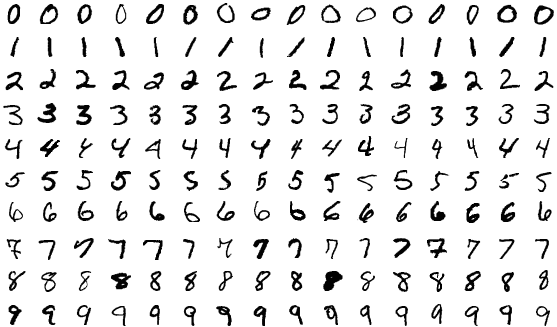
\includegraphics[scale=0.3]{Linn/MnistExamplesModified.png}
    \end{center}
    \caption{A sample of handwritten digits in the MNIST dataset. Image Credit: Wikipedia}
    \label{fig:mnist}
    \end{figure}
    

Let us try to understand this structure.
First, this subspace is a continous subspace meaning that if you take any sample and modify it in a tiny little way, it will still be recognizable as the same handwritten digit.
Second, there is connectedness, if you take any two random MNIST digits A and B, there exists a sequence of ``intermediate'' images that morph A into B in such a way that the consecutive images resemble the same digit.
This is not to say that there can't be ambiguous shapes close to the boundary between the two digits.

The technical term for such a subspace is a ``manifold''.
Just like how a smooth curve in the plane is said to be a 1D manifold within a 2D space. Because for every point on the curve, you can draw a tangent or in other words, the curve can be approximated by a line at every point.
Similiar reasons motivate you to call a smooth surface as a 2D manifold within a 3D space.
Thus to summarize the discussions so far, the \emph{manifold hypothesis} posits that all natural data lies on a low-dimensional manifold within a high-dimensional space.
This is not just true for MNIST digits, but also for human faces, the structure of galaxies, the sounds of musical instruments, and even molecular configurations.

The consequences of this manifold hypothesis is that:
    \begin{itemize}
        \item Machine learning models work in this low-dimensional highly structured subspaces within the actual input space of the problem, which can be called a latent manifold.
            This is also the kind of thing that happens when cleverly designed features are designed for seemingly difficult problem.
        \item Training data and real world data all consists of a random sampling of points from this manifold. The model then tries to interpolate between two inputs. That is, morph one into another via a continous path within the manifold.
    \end{itemize}
    This interpolation ability of machine learning models seems to be just one of the many ways to achieve generalization.
    Because humans, as we know, are capable of extreme generalization when it comes to handling everyday situations. This is without the need to be pre-trained on 
    these situations.
    This comes from our ability to reason, making use of cognitive mechanism such as abstraction, symbolic representation of the world, logic, common sense and innate priors about the world.
    \section{How to Improve Generalization}
    We saw that the ability of ML models to generalize is more of a consequence of the natural structure of the data than any property of the model itself.
    This is why the most bang for buck improvement in model performance comes from spending time with the data - cleaning data, using more informative features and removing noisy features.
    While adding more data you need to make sure that this addition is leading to a more dense sampling of the input space.
    It is when all these steps have been exhausted that you should consider model improvements.
    With regard to model and training you can do the following to maximize generalization or to avoid overfitting.
        \begin{itemize}
            \item Stop before you overfit. This involves using early stopping and saving your model to use the best possible model.
            \item Regularize your model. This involves a set of best practices to prevent your model from overfitting. The end goal is to make your model more smooth or `regular'.
        \end{itemize}
        \section{Regularization Techniques}
        If your model is overparametrized try reducing the network size. At the same time make sure that you do not go into underfitting.
        With weight regularization techniques you prefer a model that relies on a lesser number of connections.
        This is done by penalizing the magnitude of the weights propotional to the absolute magnitude (l1-regularization) or to the square of the magnitude (l2-regularization).
        However note that this doesn't have much of an effect if your model is very heavily parametrized in the first place. Hence this is much more commonly used with smaller models.
        For larger models dropout is an effective technique for regularizations.
        This involves randomly removing a different set of neurons on each example. This would impede the ability of the network to learn patterns that aren't significant.
        The dropout rate decides the number of neurons to be removed.
        \nocite{chollet_deep_2021}
\begin{thebibliography}{1}
\providecommand{\natexlab}[1]{#1}
\providecommand{\url}[1]{\texttt{#1}}
\expandafter\ifx\csname urlstyle\endcsname\relax
  \providecommand{\doi}[1]{doi: #1}\else
  \providecommand{\doi}{doi: \begingroup \urlstyle{rm}\Url}\fi

\bibitem[Chollet(2021)]{chollet_deep_2021}
Fran{\c c}ois Chollet.
\newblock \emph{Deep Learning with {{Python}}}.
\newblock Manning, Shelter Island, NY, second edition edition, 2021.
\newblock ISBN 978-1-61729-686-4.

\end{thebibliography}
    %</note>
    \printbibliography
\end{document}
